\section{Random forest}

\subsection{From-Scratch Implementation}


\subsubsection{Graphical Analysis}

\paragraph{Metric Comparison Plot}
The figure below illustrates the comparison of the
main evaluation metrics across the three resampling strategies. Tomek Links
consistently achieves the highest overall performance, particularly in terms
of accuracy and F1-score.

\begin{figure}[H]
    \centering
    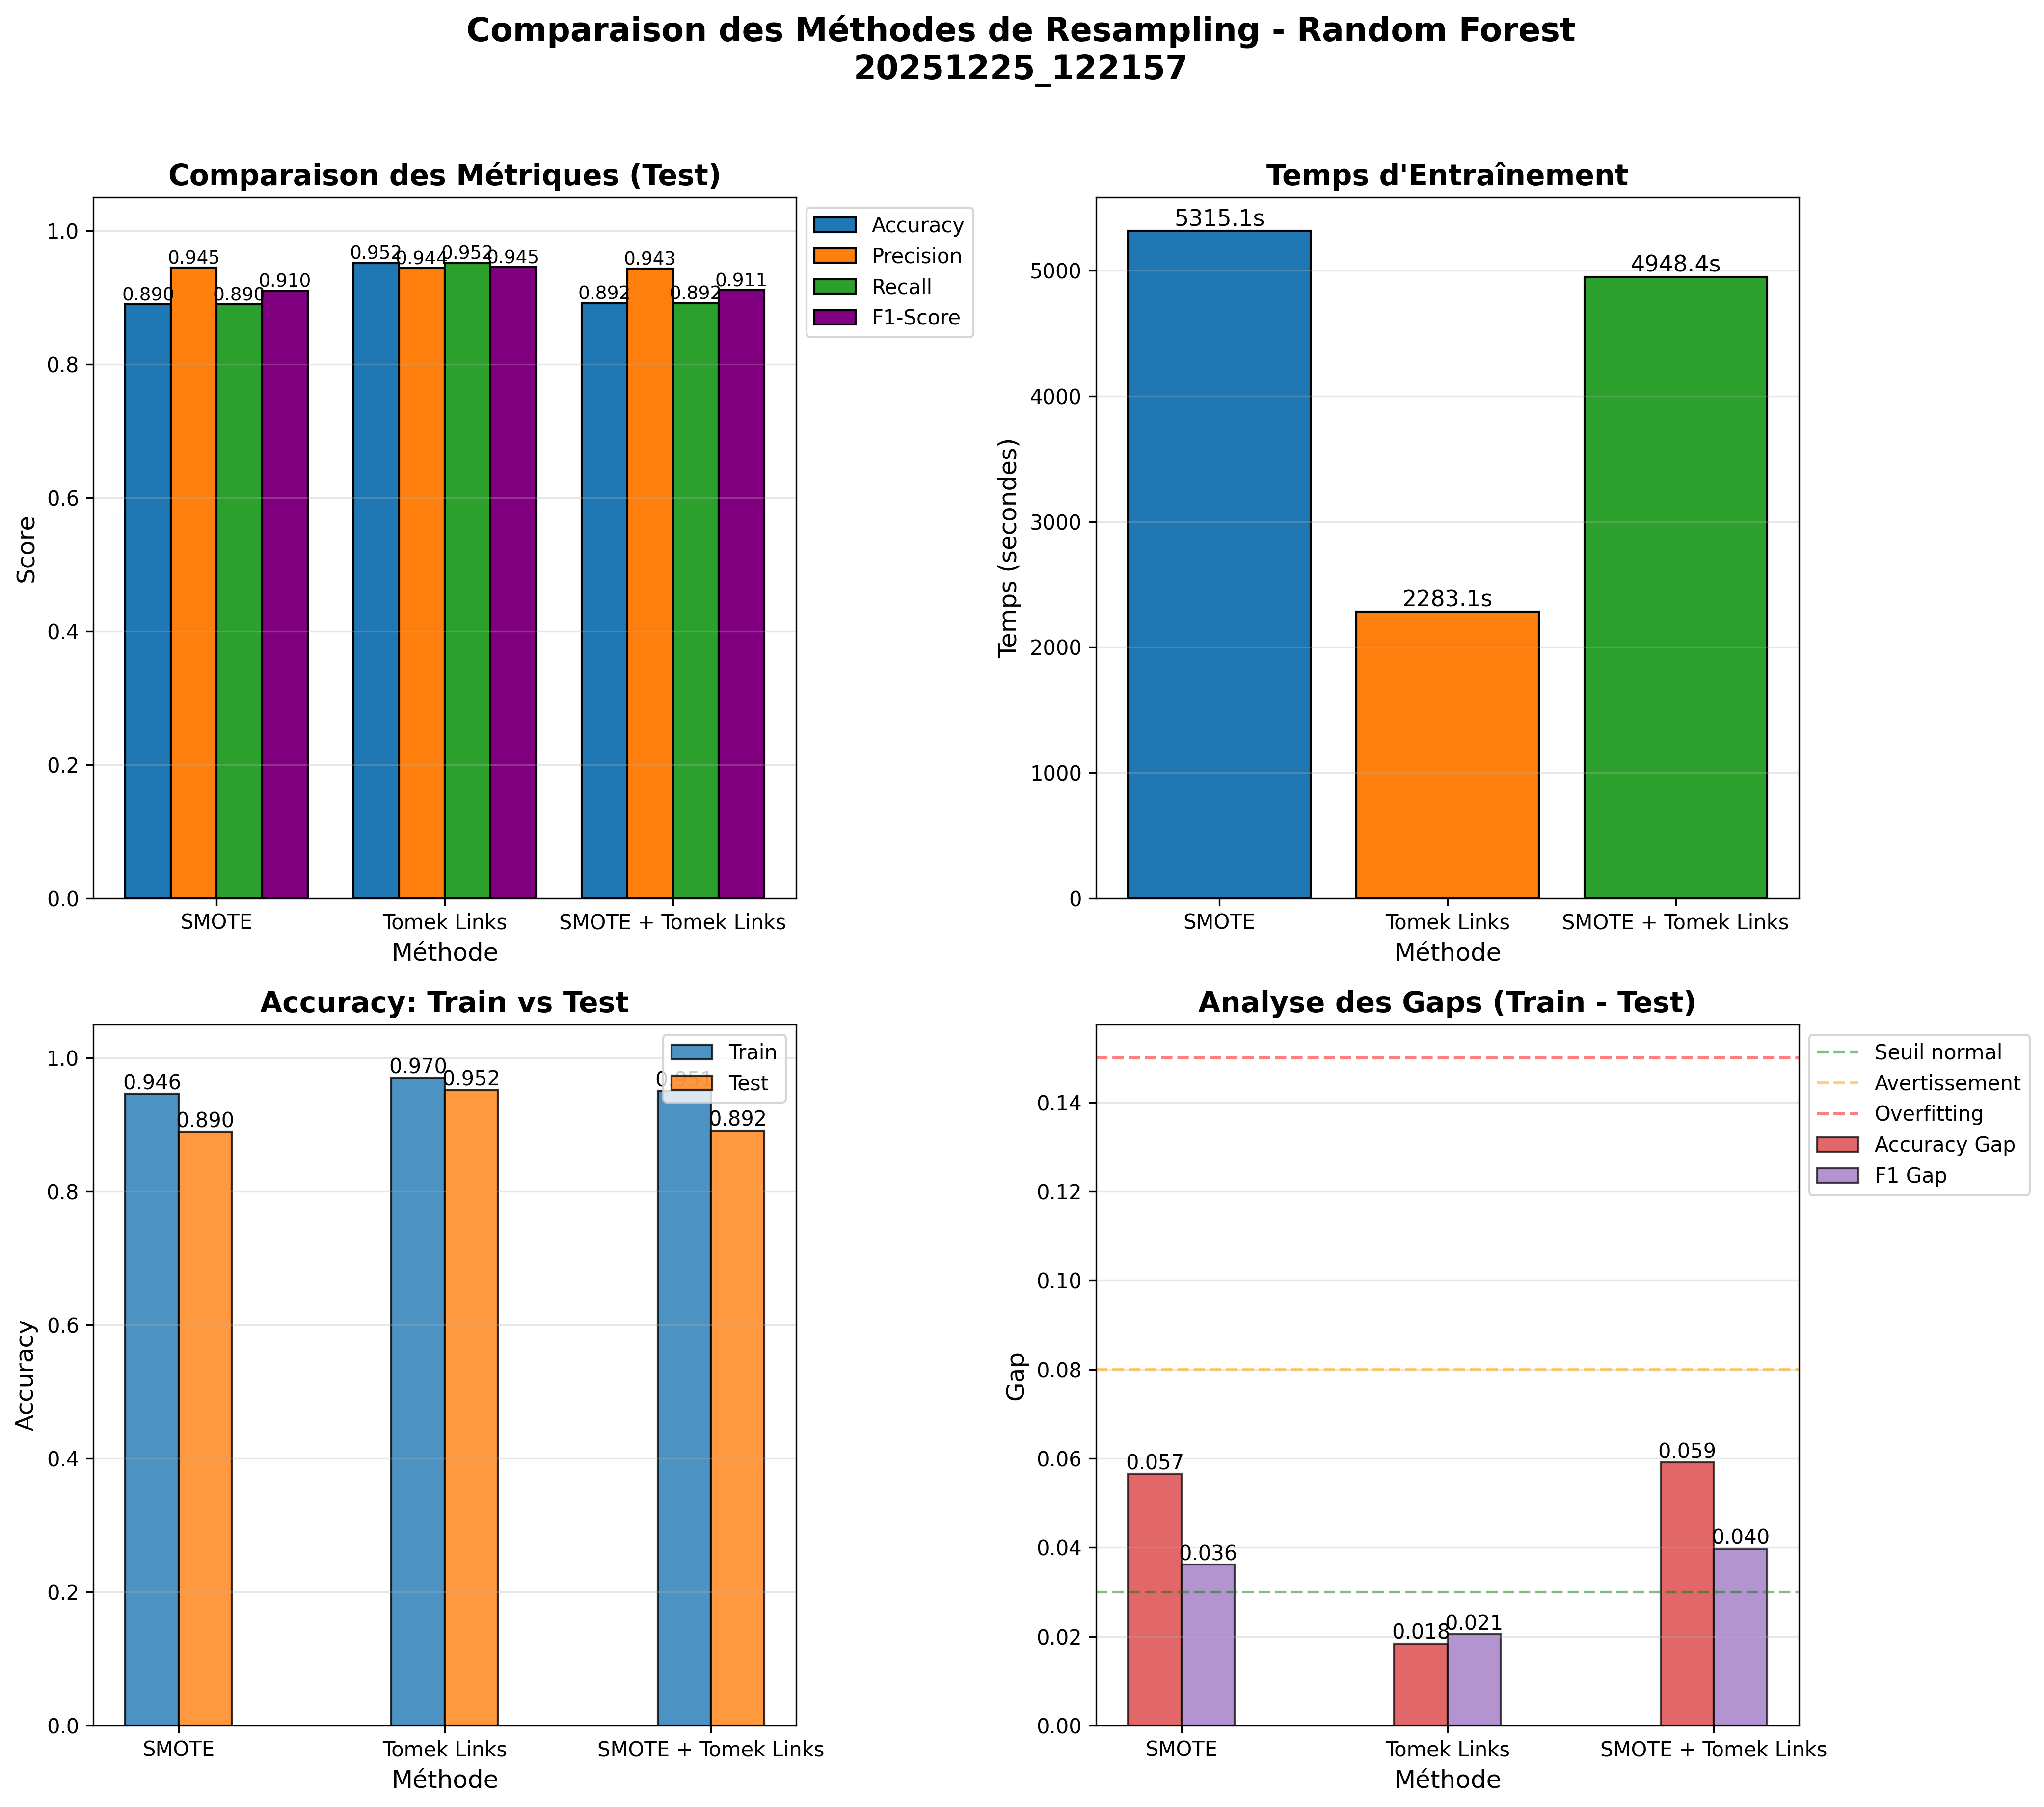
\includegraphics[width=0.7\textwidth]{images/RF/from_scratch/comparison_plot_20251225_122157.png}
    \caption{Random Forest (From Scratch) -- Comparison of Resampling Methods}
    \label{fig:rf_scratch_comparison_plot}
\end{figure}

\subsubsection{Overfitting Analysis}

The gap between training and test performance was analyzed to assess
overfitting. Tomek Links exhibits the smallest generalization gap
(\textbf{Accuracy gap = 0.0185}, \textbf{F1 gap = 0.0205}), indicating excellent
generalization compared to SMOTE-based approaches, which show mild
overfitting.

\paragraph{Radar Chart Analysis}
The radar chart below provides a holistic view of
the trade-offs between precision, recall, F1-score, accuracy, and computational
cost. Tomek Links demonstrates the best balance between predictive performance
and training time (biggest and roundest polygon).

\begin{figure}[H]
    \centering
    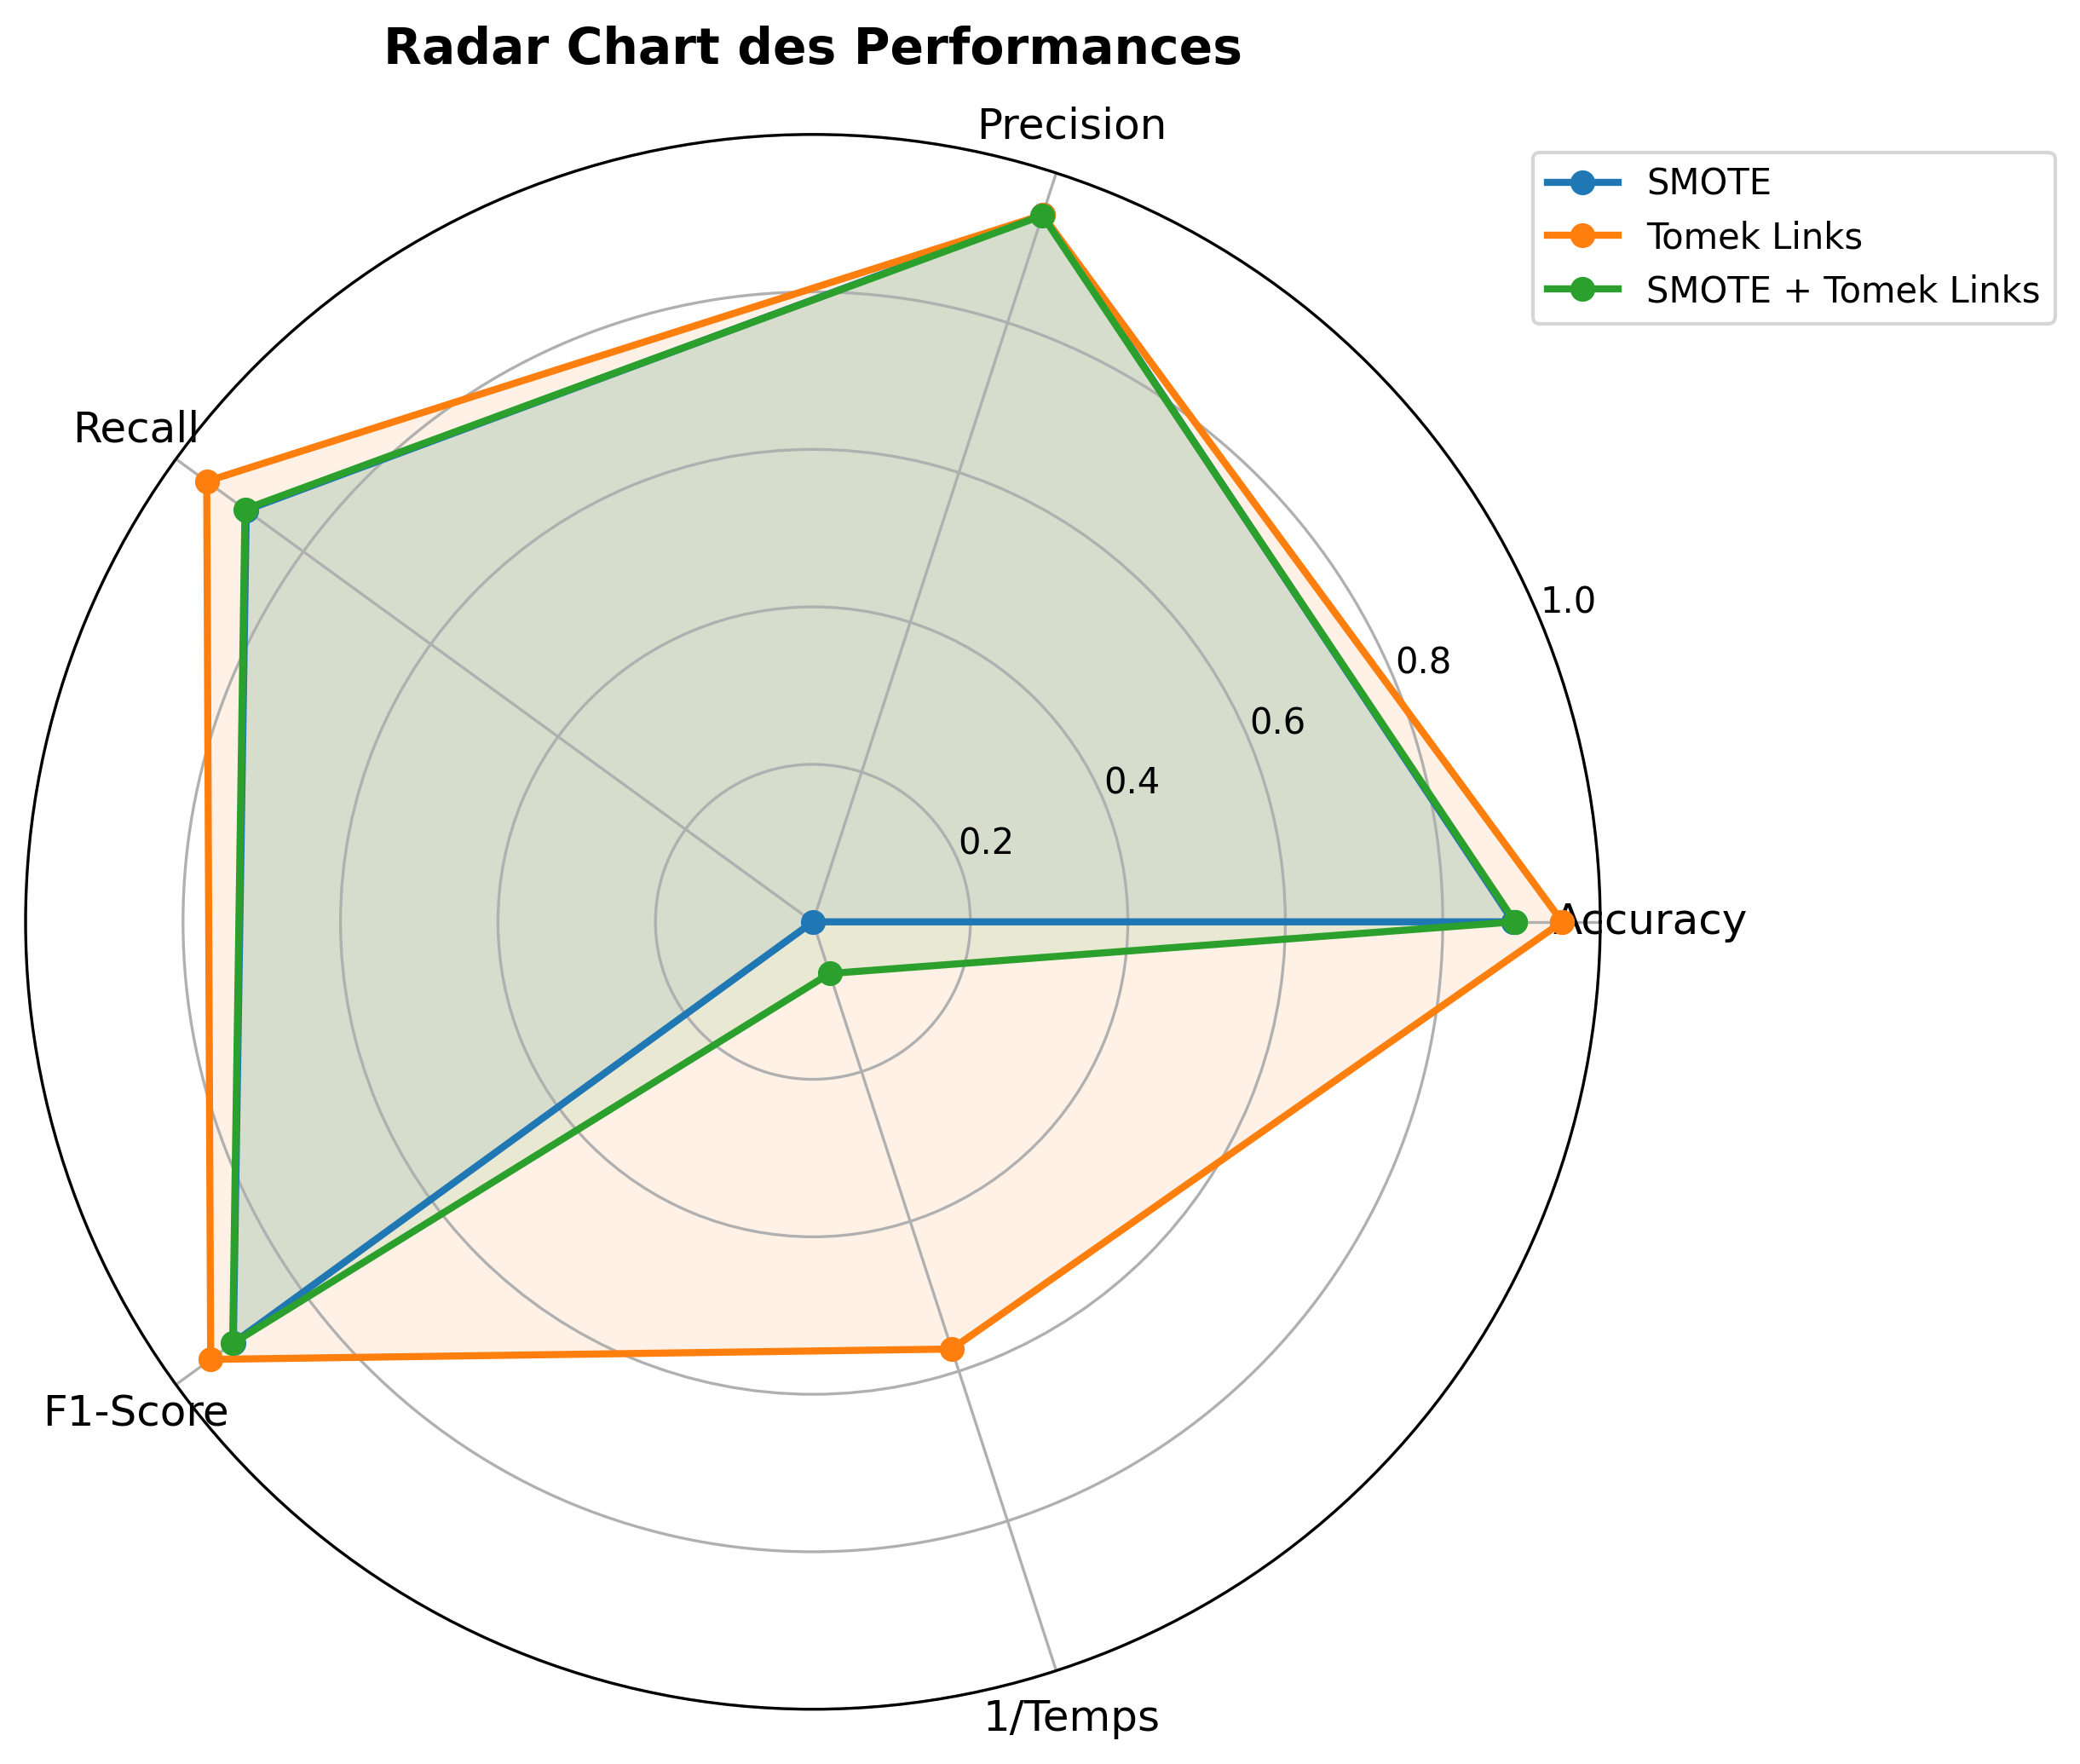
\includegraphics[width=0.5\textwidth]{images/RF/from_scratch/radar_chart_20251225_122157.png}
    \caption{Random Forest (From Scratch) -- Radar Chart Comparison}
    \label{fig:rf_scratch_radar}
\end{figure}




\subsection{Scikit-learn Implementation}


\begin{table}[H]
\centering
\caption{Scikit-Learn Random Forest Class-wise Precision and Recall}
% \label{tab:rf_precision_recall}
\begin{tabular}{|l|c|c|c|c|}
\hline
\textbf{Resampling} & \textbf{Class 0 Precision} & \textbf{Class 0 Recall} & \textbf{Class 1 Precision} & \textbf{Class 1 Recall} \\ \hline
SMOTE & 0.98 & 0.91 & 0.33 & 0.68 \\ \hline
Tomek & 0.96 & 0.98 & 0.57 & 0.36 \\ \hline
SMOTE-Tomek & 0.98 & 0.91 & 0.31 & 0.66 \\ \hline
\end{tabular}
\end{table}



\subsection{Bayesian Optimization for Random Forest}

Bayesian Optimization was used to tune Random Forest hyperparameters on the SMOTE-Tomek dataset. The search space included \texttt{n\_estimators} (50–200), \texttt{max\_depth} (5–25), and \texttt{max\_features} (0.1–0.9).

\begin{table}[H]
\centering
\caption{Selected Iterations from Bayesian Optimization for Random Forest}
\label{tab:rf_bayes_iterations}
\begin{tabular}{|c|c|c|c|c|}
\hline
\textbf{Iteration} & \textbf{CV Accuracy} & \textbf{n\_estimators} & \textbf{max\_depth} & \textbf{max\_features} \\ \hline
1  & 0.9691 & 106 & 24.01 & 0.686 \\ 
3  & 0.9678 & 59  & 22.32 & 0.581 \\ 
6  & 0.9695 & 109 & 24.21 & 0.636 \\ 
10 & 0.9703 & 71  & 25.00 & 0.100 \\ 
16 & 0.9710 & 175 & 25.00 & 0.100 \\ 
19 & 0.9710 & 159 & 25.00 & 0.100 \\ \hline
\end{tabular}
\end{table}

Bayesian Optimization completed in approximately 419 seconds. The optimal hyperparameters were \texttt{n\_estimators}=159, \texttt{max\_depth}=25, \texttt{max\_features}=0.1, \texttt{random\_state}=42, and \texttt{n\_jobs}=-1.

\subsection{Discussion}

The Random Forest classifier achieved consistently high performance on the majority class (Class 0) across all resampling strategies, with SMOTE slightly improving minority class recall. Bayesian optimization further improved validation accuracy, achieving 0.9336 on the SMOTE-Tomek dataset. Training times were reasonable, and Random Forest proved to be robust for handling class imbalance in forest fire prediction tasks.
